\documentclass[unicode,11pt,a4paper,oneside,numbers=endperiod,openany]{scrartcl}
\usepackage{amsmath}
\usepackage{amssymb}
\usepackage{enumitem}
\usepackage{multicol}
\usepackage{ifthen}
\usepackage[utf8]{inputenc}
\usepackage{graphics}
\usepackage{graphicx}
\usepackage{hyperref}

\pagestyle{plain}
\voffset -5mm
\oddsidemargin  0mm
\evensidemargin -11mm
\marginparwidth 2cm
\marginparsep 0pt
\topmargin 0mm
\headheight 0pt
\headsep 0pt
\topskip 0pt        
\textheight 255mm
\textwidth 165mm

\newcommand{\duedate} {}
\newcommand{\setduedate}[1]{%
\renewcommand\duedate {Due date:~ #1}}
\newcommand\isassignment {false}
\newcommand{\setassignment}{\renewcommand\isassignment {true}}
\newcommand{\ifassignment}[1]{\ifthenelse{\boolean{\isassignment}}{#1}{}}
\newcommand{\ifnotassignment}[1]{\ifthenelse{\boolean{\isassignment}}{}{#1}}

\newcommand{\assignmentpolicy}{
\begin{table}[h]
\begin{center}
\scalebox{0.8} {%
\begin{tabular}{|p{0.02cm}p{16cm}|}
\hline
&\\
\multicolumn{2}{|c|}{\Large\textbf{HPC Lab for CSE 2024 ---  Submission Instructions}}\\
\multicolumn{2}{|c|}{\large\textbf{(Please, notice that following instructions are mandatory: }}\\
\multicolumn{2}{|c|}{\large\textbf{submissions that don't comply with, won't be considered)}}\\
&\\
\textbullet & Assignments must be submitted to \href{https://moodle-app2.let.ethz.ch/course/view.php?id=22516}{Moodle} (i.e. in electronic format).\\
\textbullet & Provide both executable package and sources (e.g. C/C++ files, Matlab). 
If you are using libraries, please add them in the file. Sources must be organized in directories called:\\
\multicolumn{2}{|c|}{\textit{Project\_number\_lastname\_firstname}}\\
& and  the  file must be called:\\
\multicolumn{2}{|c|}{\textit{project\_number\_lastname\_firstname.zip}}\\
\multicolumn{2}{|c|}{\textit{project\_number\_lastname\_firstname.pdf}}\\
\textbullet &  The TAs will grade your project by reviewing your project write-up, and looking at the implementation 
                 you attempted, and benchmarking your code's performance.\\

\textbullet & You are allowed to discuss all questions with anyone you like; however: (i) your submission must list anyone you discussed problems with and (ii) you must write up your submission independently.\\
\hline
\end{tabular}
}
\end{center}
\end{table}
}
\newcommand{\punkte}[1]{\hspace{1ex}\emph{\mdseries\hfill(#1~\ifcase#1{Points}\or{Points}\else{Points}\fi)}}


\newcommand\serieheader[6]{
\thispagestyle{empty}%
\begin{flushleft}

\includegraphics[width=0.4\textwidth]{ETHlogo_13}
\end{flushleft}
  \noindent%
  {\large\ignorespaces{\textbf{#1}}\hspace{\fill}\ignorespaces{ \textbf{#2}}}\\ \\%
  {\large\ignorespaces #3 \hspace{\fill}\ignorespaces #4}\\
  \noindent%
  \bigskip
  \hrule\par\bigskip\noindent%
  \bigskip {\ignorespaces {\Large{\textbf{#5}}}
  \hspace{\fill}\ignorespaces \large \ifthenelse{\boolean{\isassignment}}{\duedate}{#6}}
  \hrule\par\bigskip\noindent%  \linebreak
 }

\makeatletter
\def\enumerateMod{\ifnum \@enumdepth >3 \@toodeep\else
      \advance\@enumdepth \@ne
      \edef\@enumctr{enum\romannumeral\the\@enumdepth}\list
      {\csname label\@enumctr\endcsname}{\usecounter
        {\@enumctr}%%%? the following differs from "enumerate"
	\topsep0pt%
	\partopsep0pt%
	\itemsep0pt%
	\def\makelabel##1{\hss\llap{##1}}}\fi}
\let\endenumerateMod =\endlist
\makeatother




\usepackage{textcomp}






\begin{document}


\setassignment
\setduedate{Wednesday 26 June 2024, 23:59}

\serieheader{AI in the Sciences and Engineering}{Spring Semester 2024}
            {Student: Carla Judith L\'opez Zurita}
            {}{Project 3}{}
\newline

The main objective of the project is to apply the concepts learned in class
related to Neural Differential Equations and Hybrid Workflows, as well Model
Discovery. The project is divided into two tasks.


\section{Inverted pendulum}\label{sec:task1}
The objective of the first task is to control the inverted pendulum problem using a
Neural Network. This is to be achieved by applying an 
external force $F$ to the cart that holds the pendulum, which is free to move
horizontally.
The system is described by the following differential equation:
\begin{align}
    (M+m) \ddot{x} + m l \ddot{\theta} \cos(\theta) - m l \dot{\theta}^2 \sin(\theta) = F, \\
    l \ddot{\theta} + g \sin(\theta) + \ddot{x} \cos(\theta) = 0,
\end{align}
where $\theta$ is the angle of the pendulum with respect to the vertical,
$g=9.81$ m/s$^2$ is the acceleration due to gravity, $l=1.0$ m is the length of
the pendulum, $m=0.1$ kg is the mass of the pendulum, $M=1.0$ kg is the mass of
the cart and $F$ is the force applied to the cart in Newtons.

\subsection*{Solving the coupled ODE system}
First, we need to solve the coupled ODE system and simulate the dynamics of the
inverted pendulum.
The idea is to use an autodifferentiation library to code the solver in order to
be able to use it in the Neural Network training process. 
For my implementation, I chose \texttt{pytorch} due to its familiarity to me.
As integration scheme, I used Runge-Kutta 4th order method. To test the
code, I simulated the system with a sinusoidal force $F(t) = 10
\sin(t)$.
The results are shown in Figure~\ref{fig:pendulum} in the Appendix~\ref{app:pendulum}.

\subsection*{Learning to balance the pendulum}
Next, we will implement the Neural Network trainer.
The input to the network is time $t$ and the output is the force $F$ applied to
the cart. 
The network is trained using the whole trajectory of the pendulum, with the
Adam optimizer and a custom loss function that penalizes the deviation of the
pendulum from the vertical position and large angular velocities. 
The network is a simple feedforward network with
1 hidden layer with 32 neurons and SiLU activation function. The output layer
has a single neuron with linear activation function. The network is trained for
500 epochs with an initial learning rate of $10^{-2}$ and a scheduler that
reduces the learning rate by a factor of 0.5 every 75 epochs.
The plot of the loss function during training is shown in Figure~\ref{fig:loss}.

\begin{figure}[h!]
    \hspace*{-1cm}
    \centering
    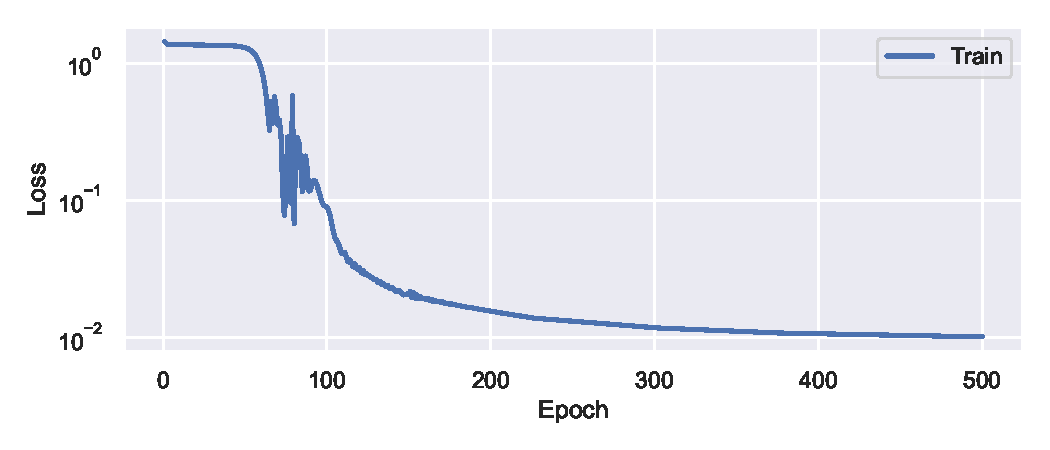
\includegraphics[width=0.8\textwidth]{../Task1/loss_function.pdf}
    \caption{Loss function during training of the Neural Network.}
    \label{fig:loss}
\end{figure}
The results of the simulation using the Neural Network to control the force
applied to the cart are shown in Figure~\ref{fig:pendulum_nn}.
Attatched to the report you will find the code used to solve the ODE system and
train the Neural Network, as well as the simulation results in a \texttt{gif} format.
\begin{figure}[h!]
    \centering
    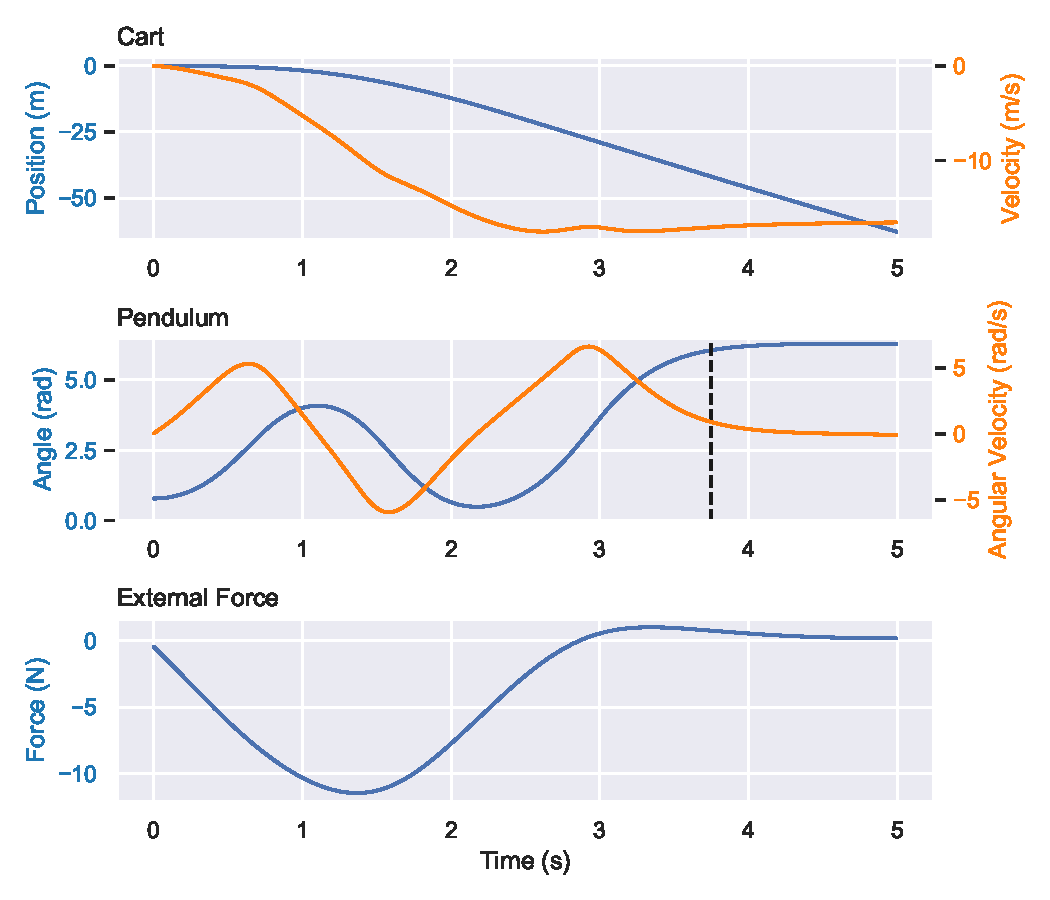
\includegraphics[width=0.85\textwidth]{../Task1/pendulum_nn.pdf}
    \caption{Simulation of the inverted pendulum using a Neural Network to
    control the force applied to the cart.}
    \label{fig:pendulum_nn}
\end{figure}

\newpage
\section{Model discovery}\label{sec:task2}
The objective of this task is to write our own PDE-FIND~\cite{PDEFIND} algorithm to discover the
differential equation that governs the dynamics of the some unkown system using
only provided data files.

Based on the assumption that the dynamics of the system can be described
by a partial differential equation of the form
\begin{align}\label{eq:pde}
    u_t = F(u, u_x, u_{xx}, u_y, u_{yy}, u_{xy}, \ldots, x, y, \ldots, t),
\end{align}
we can create a library of possible functions that can appear in the right
hand side of the equation,
\begin{align}\label{eq:library}
    \Theta(\mathbf{u}) = [ \mathbf{u}, \mathbf{u}_x, \mathbf{u}_{xx}, \mathbf{u}_y, \mathbf{u}_{yy}, \mathbf{u}_{xy}, \mathbf{u}\mathbf{u}_x, \mathbf{u}\mathbf{u}_y, \ldots ].
\end{align}
We then use the given data to find the coefficients $\xi$ of the
functions that best describe the dynamics of the system,
\begin{align}\label{eq:coefficients}
    \mathbf{u}_t = \Theta(\mathbf{u})\xi.
\end{align}
For the task, we are given three files with data of differents system in order of increasing complexity.

\subsection*{Implementation of PDE-FIND}
My implementation of the PDE-FIND consists on using finite difference scheme,
taken directly from the \texttt{pysindy} library, to compute the partial derivatives.
\cite{PDEFIND}. It uses centered differences, with consideration of the boundary conditions.
I used it recursively to compute the second and third order
mixed derivatives.
To build the library of possible functions, I included linear and non-linear
combinations of the computed derivatives, excluding
the time and space coordinates as possible functions. I also excluded
derivatives that include time.
Finally, I used LassoCV from the \texttt{scipy} library to find the coefficients of the functions as in
Equation~\eqref{eq:coefficients}. Finally,
coefficients that are below a certain threshold ($10^{-2}$) are removed.


\subsection*{File 1}
The first file is a 1+1D dimensional system with dependent variable $u$, and
independent variables $x$ and $t$ as coordinates.
% Figure~\ref{fig:data1} shows the data of the first file, accompanied by its temporal
% derivative computed using the finite difference scheme.
% \begin{figure}[h]\label{fig:data1}
%     \centering
%     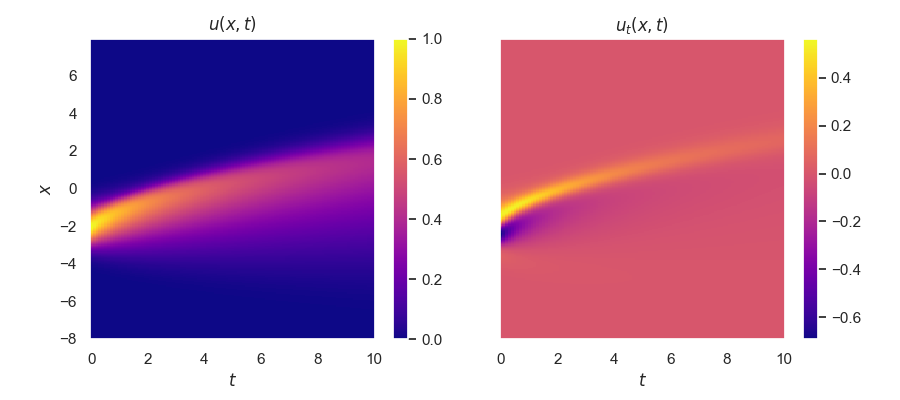
\includegraphics[width=0.8\textwidth]{../Task2/figures/data_1.png}
%     \caption{Data of the first file, with its temporal derivative.}
% \end{figure}
We can then build the library of possible functions as in
Equation~\eqref{eq:library}, using the partial derivatives in $x$ up to
third order.
The library of possible functions is shown in Equation~\eqref{eq:library1},
which includes 15 terms.
\begin{align}\label{eq:library1}
    \Theta(\mathbf{u}) = [ \mathbf{u}, \mathbf{u}_x, \mathbf{u}_{xx}, \mathbf{u}_{xxx}, \mathbf{u}\mathbf{u}, \mathbf{u} \mathbf{u}_x, \mathbf{u} \mathbf{u}_{xx}, \mathbf{u} \mathbf{u}_{xxx}, \mathbf{u}_x \mathbf{u}_x, \mathbf{u}_x \\
    % no number for the last line
    \mathbf{u}_{xx}, \mathbf{u}_x \mathbf{u}_{xxx}, \mathbf{u}_{xx} \mathbf{u}_{xx}, \mathbf{u}_{xx} \mathbf{u}_{xxx}, \mathbf{u}_{xxx} \mathbf{u}_{xxx}, \mathbf{u}\mathbf{u}\mathbf{u} ]. \nonumber
\end{align}
The PDE-FIND algorithm was fitted using the \texttt{LassoCV} regression
technique with following parameters
\begin{verbatim}
    LassoCV(alphas=[1e-6, 1e-5], fit_intercept=False,
            cv=3, tol=1e-6, max_iter=int(1e8))
\end{verbatim}
The results of the PDE-FIND algorithm are
\begin{align}
    %	-1.0u*u_x + 0.1u_xx = u_t
    \mathbf{u}_t = -1.0 \mathbf{u} \mathbf{u}_x + 0.1 \mathbf{u}_{xx}.
\end{align}
which let us know that the system is governed by Burger's equation.
Figure 4 in the Appendix~\ref{app:resultsall}
shows the prediction of the system using the
discovered PDE and the difference between the prediction and the actual data.
The prediction is very good, and has a
mean squared error of 5.5729e-07. The discovered PDE is theoretically correct.

\subsection*{File 2}
The second file is also a 1+1D dimensional system $u(t, x)$. The same
type of derivatives and library terms are used as in the previous case, shown in
Equation~\eqref{eq:library1}.
% Figure~\ref{fig:data2} shows the data of the second file, with its temporal derivative.
% \begin{figure}[h]\label{fig:data2}
%     \centering
%     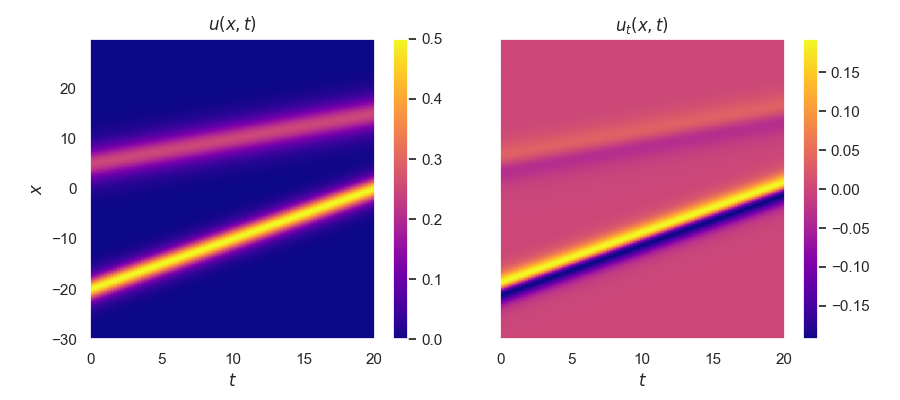
\includegraphics[width=0.8\textwidth]{../Task2/figures/data_2.png}
%     \caption{Data of the second file, with its temporal derivative.}
% \end{figure}
To fit the model, I also used the same parameters.
The results of the PDE-FIND algorithm are
\begin{align}
    % 	-5.4u*u_x + -0.9u_xxx + -0.11u_x*u_xx + -0.081u_x = u_t
    \mathbf{u}_t = -5.4 \mathbf{u} \mathbf{u}_x - 0.9 \mathbf{u}_{xxx} - 0.11 \mathbf{u}_x \mathbf{u}_{xx} - 0.081 \mathbf{u}_x,
\end{align}
which imply that the system is governed by the
Korteweg-de Vries equation, choosing to ignore the terms $\mathbf{u}_x \mathbf{u}_{xx}$ and
$\mathbf{u}_x$. Since this file is a bit more complex, the algorithm is not able
to find the exact equation. 
Figure 5 in the Appendix~\ref{app:resultsall} shows the numerical prediction of the system.
The mean squared error is 1.4913e-06, which is higher than in the previous case.
Perhaps using a finer grid could help to improve the
results due to the higher order derivatives.

\subsection*{File 3}
The final file is a 2+1D dimensional system, with $x$, $y$ and $t$ coordinates, where the solution is a vector
field with two components, $u(x, t)$ and $v(x, t)$. In this case the PDE is a set of two coupled
equations of the form
\begin{align}
    % ut = D1(u, ux, v, vx, uv, ...),
    % vt = D2(u, ux, v, vx, uv, ...).
    \mathbf{u}_t & = \mathcal{D}_1(\mathbf{u}, \mathbf{u}_x, \mathbf{v}, \mathbf{v}_x, \mathbf{u} \mathbf{v}, \ldots), \\
    \mathbf{v}_t & = \mathcal{D}_2(\mathbf{u}, \mathbf{u}_x, \mathbf{v}, \mathbf{v}_x, \mathbf{u} \mathbf{v}, \ldots). \nonumber
\end{align}
% Figures~\ref{fig:data3_u} and ~\ref{fig:data3_v} shows the data of the third
% file at a given instance, with the corresponding temporal derivatives.
% \begin{figure}[h]\label{fig:data3_u}
%     \centering
%     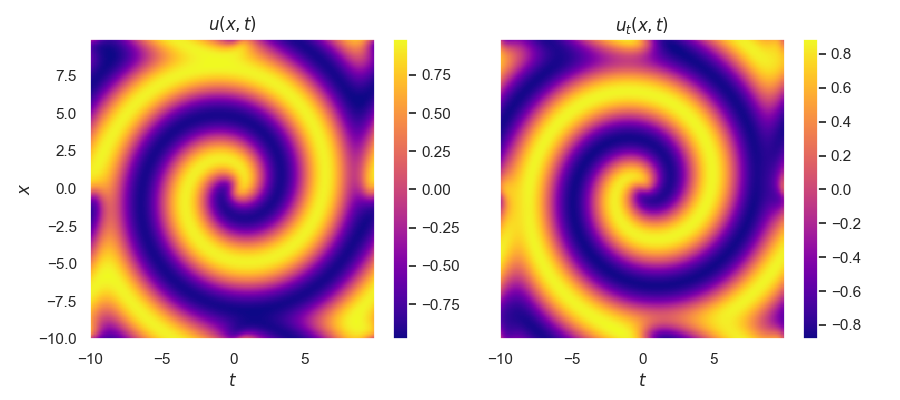
\includegraphics[width=0.8\textwidth]{../Task2/figures/data_u_3.png}
%     \caption{Data of the third file at a given $t_n$, with its temporal derivative for the first variable.}
% \end{figure}
% \begin{figure}[h]\label{fig:data3_v}
%     \centering
%     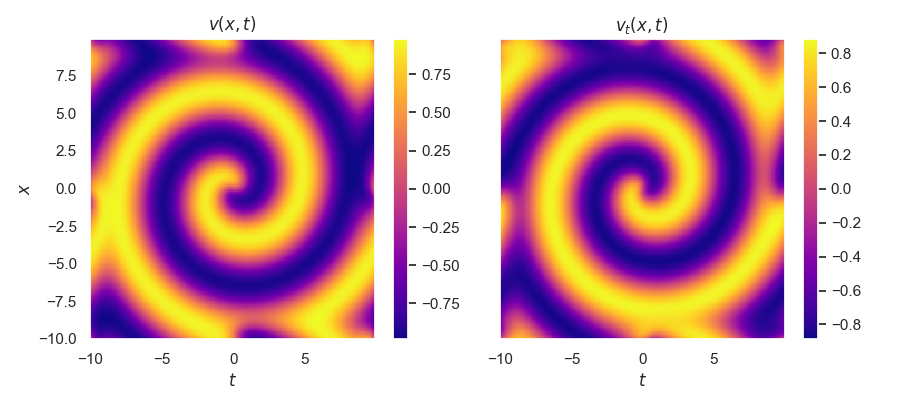
\includegraphics[width=0.8\textwidth]{../Task2/figures/data_v_3.png}
%     \caption{Data of the third file at a given $t_n$, with its temporal derivative for the second variable.}
% \end{figure}
This time, the library of possible functions includes the 52 terms, as shown in
the Appendix~\ref{app:terms3}. 
To achieve fast computation, I decided to
subsample the data along the temporal coordinate. 
I used
similar parameters for the regression as in the previous cases, and solved for the two equations separately.
The results of the PDE-FIND algorithm are
\begin{align}
    %       0.85v*v*v + 0.85u*u*v + 0.62u + -0.6u*u*u + -0.6u*v*v + 0.13v +
    %       0.085u_xx + 0.081u_yy = u_t
    \mathbf{u}_t &= 0.85 \mathbf{v}^3 + 0.85 \mathbf{u}^2 \mathbf{v} + 0.62 \mathbf{u} - 0.6 \mathbf{u}^3 - 0.6 \mathbf{u} \mathbf{v}^2 + 0.13 \mathbf{v} + 0.085 \mathbf{u}_{xx} + 0.081 \mathbf{u}_{yy}, \\
    %       -0.85u*u*u + -0.85u*v*v + 0.62v + -0.6v*v*v + -0.6u*u*v + -0.13u + 0.085v_yy + 0.081v_xx = v_t
    \mathbf{v}_t &= -0.85 \mathbf{u}^3 - 0.85 \mathbf{u} \mathbf{v}^2 + 0.62 \mathbf{v} - 0.6 \mathbf{v}^3 - 0.6 \mathbf{u}^2 \mathbf{v} - 0.13 \mathbf{u} + 0.085 \mathbf{v}_{yy} + 0.081 \mathbf{v}_{xx}.
\end{align}
We can infer that the system is a reaction-diffusion system,
\begin{align}
    % $$u_t = 0.1\nabla^2 u + (1-A^2)u +\beta A^2v$$
    % $$v_t = 0.1\nabla^2 v - \beta A^2 u + (1-A^2)v$$
    % $$A^2 = u^2 + v^2.$$
    \mathbf{u}_t &= 0.1 \nabla^2 \mathbf{u} + (1 - A^2) \mathbf{u} + \beta A^2 \mathbf{v}, \\
    \mathbf{v}_t &= 0.1 \nabla^2 \mathbf{v} - \beta A^2 \mathbf{u} + (1 - A^2) \mathbf{v}, \\
    A^2 &= \mathbf{u}^2 + \mathbf{v}^2.
\end{align}
The algorithm is not able to find the exact equation, and it gives coefficients
for some extra terms
($0.13v$ and $0.62u$), and also not the exact coefficients for the rest of the
terms.
Figures 6 and 7 in the Appendix~\ref{app:resultsall}
show the prediction of the system.
The prediction is not as good as in the previous cases, reaching a mean
squared error of 7.1573e-05 for the first variable and 7.1707e-05 for the
second, 
but it still captures the dynamics of the system and discovers
the correct type of equation. A higher error could be due to the complexity of the system and the noise
in the data. Higher convergence could be achieved by a lower subsampling rate,
but at the cost of higher computational time.

\bibliographystyle{plain}
\bibliography{bibliography}


% \section{Transfer learning}\label{sec:task3}
\newpage
\appendix
\section {Inverted pendulum with a sinusoidal force}\label{app:pendulum}
The results of the simulation of the inverted pendulum with a sinusoidal force are shown in Figure~\ref{fig:pendulum}.
\begin{figure}[h!]
    \centering
    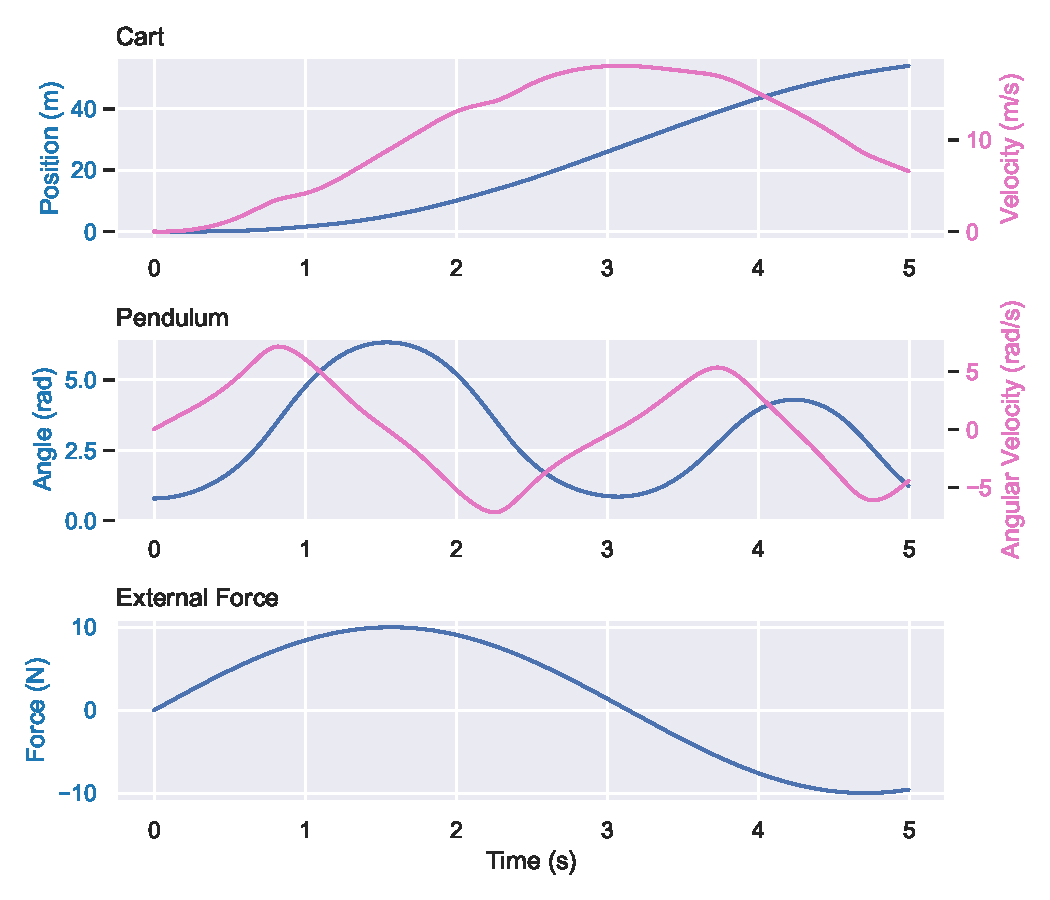
\includegraphics[width=0.85\textwidth]{../Task1/pendulum.pdf}
    \caption{Simulation of the inverted pendulum with a sinusoidal force.}
    \label{fig:pendulum}
\end{figure}

\section{Numerical results of PDE-FIND}\label{app:resultsall}
Attatched are the figures corresponding to the results of the PDE-FIND algorithm for
all files.

\begin{figure}[h!]\label{fig:results1}
    \centering
    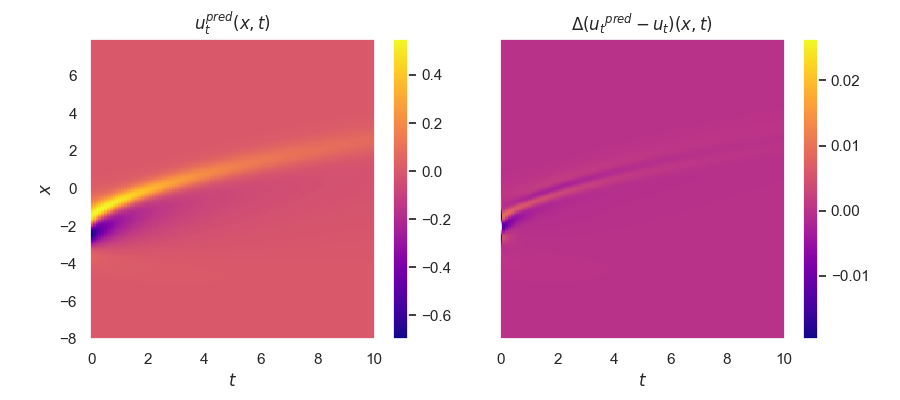
\includegraphics[width=0.8\textwidth]{../Task2/figures/results_1.png}
    \caption{Prediction of the first file using the discovered PDE.
    MSE: 5.5729e-07.
    }
\end{figure}

\begin{figure}[h!]\label{fig:results2}
    \centering
    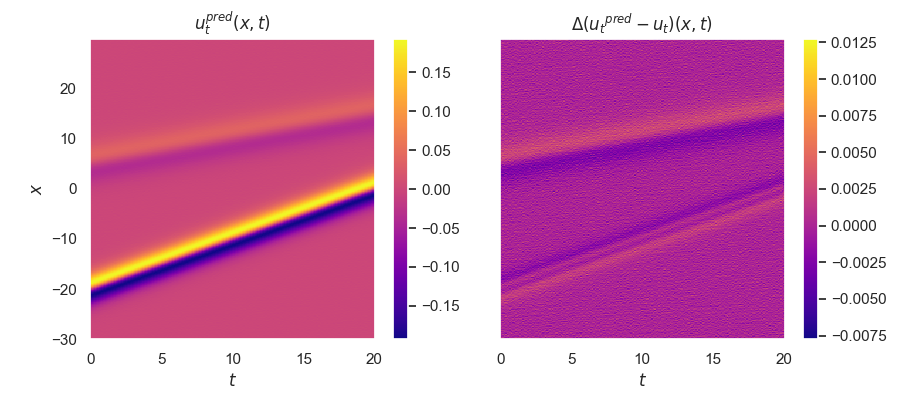
\includegraphics[width=0.8\textwidth]{../Task2/figures/results_2.png}
    \caption{Prediction of the second file using the discovered PDE. MSE: 1.4913e-06
    }
\end{figure}

\begin{figure}[h!]\label{fig:results_u_3}
    \centering
    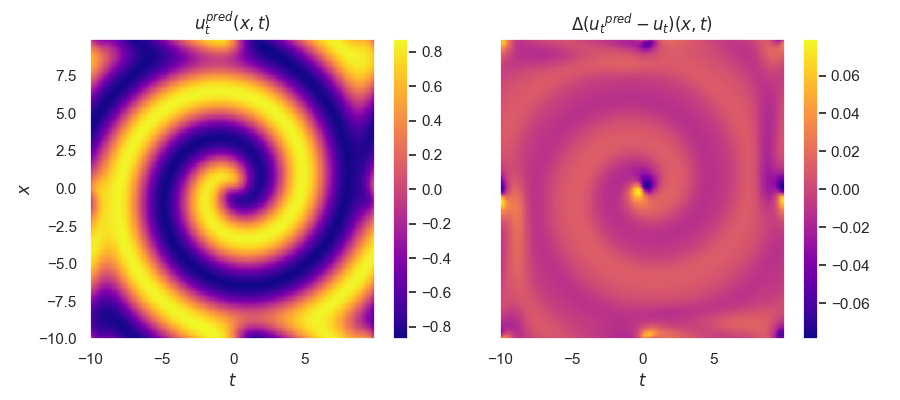
\includegraphics[width=0.8\textwidth]{../Task2/figures/results_u_3.png}
    \caption{Prediction of the third file for $u$ using the discovered PDE. MSE: 7.1573e-05.}
\end{figure}
\begin{figure}[h!]\label{fig:results_v_3}
    \centering
    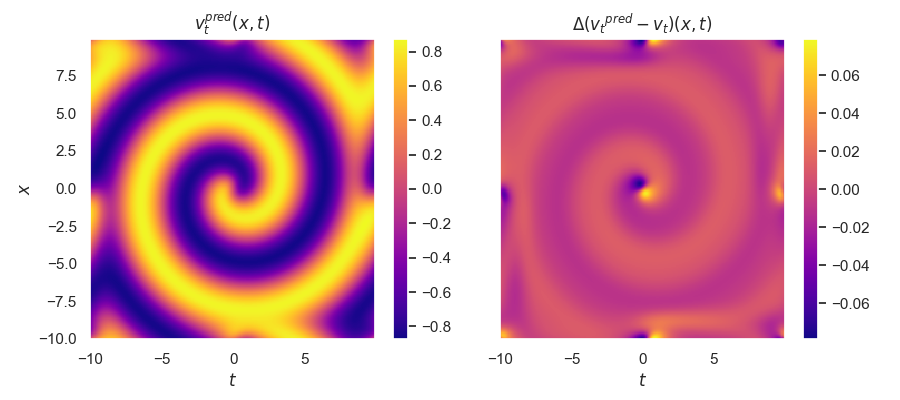
\includegraphics[width=0.8\textwidth]{../Task2/figures/results_v_3.png}
    \caption{Prediction of the third file for the $v$ using the discovered PDE. MSE: 7.1707e-05.}
\end{figure}

\newpage
\section{Library of possible functions for File 3}\label{app:terms3}
The library of possible functions for the third file is shown below.
\begin{multicols}{5}
\begin{itemize}[noitemsep, topsep=0pt, left=0pt]
    \item $\mathbf{u}$
    \item $\mathbf{v}$
    \item $\mathbf{u}_{x}$
    \item $\mathbf{u}_{xx}$
    \item $\mathbf{u}_{xxx}$
    \item $\mathbf{u}_{xxy}$
    \item $\mathbf{u}_{xy}$
    \item $\mathbf{u}_{xyx}$
    \item $\mathbf{u}_{xyy}$
    \item $\mathbf{u}_{y}$
    \item $\mathbf{u}_{yy}$
    \item $\mathbf{u}_{yyx}$
    \item $\mathbf{u}_{yyy}$
    \item $\mathbf{v}_{x}$
    \item $\mathbf{v}_{xx}$
    \item $\mathbf{v}_{xxx}$
    \item $\mathbf{v}_{xxy}$
    \item $\mathbf{v}_{xy}$
    \item $\mathbf{v}_{xyx}$
    \item $\mathbf{v}_{xyy}$
    \item $\mathbf{v}_{y}$
    \item $\mathbf{v}_{yy}$
    \item $\mathbf{v}_{yyx}$
    \item $\mathbf{v}_{yyy}$
    \item $\mathbf{u} \mathbf{u}$
    \item $\mathbf{v} \mathbf{v}$
    \item $\mathbf{u}_{x} \mathbf{u}_{x}$
    \item $\mathbf{u}_{xx} \mathbf{u}_{xx}$
    \item $\mathbf{u}_{xxx} \mathbf{u}_{xxx}$
    \item $\mathbf{u}_{xxy} \mathbf{u}_{xxy}$
    \item $\mathbf{u}_{xy} \mathbf{u}_{xy}$
    \item $\mathbf{u}_{xyx} \mathbf{u}_{xyx}$
    \item $\mathbf{u}_{xyy} \mathbf{u}_{xyy}$
    \item $\mathbf{u}_{y} \mathbf{u}_{y}$
    \item $\mathbf{u}_{yy} \mathbf{u}_{yy}$
    \item $\mathbf{u}_{yyx} \mathbf{u}_{yyx}$
    \item $\mathbf{u}_{yyy} \mathbf{u}_{yyy}$
    \item $\mathbf{v}_{x} \mathbf{v}_{x}$
    \item $\mathbf{v}_{xx} \mathbf{v}_{xx}$
    \item $\mathbf{v}_{xxx} \mathbf{v}_{xxx}$
    \item $\mathbf{v}_{xxy} \mathbf{v}_{xxy}$
    \item $\mathbf{v}_{xy} \mathbf{v}_{xy}$
    \item $\mathbf{v}_{xyx} \mathbf{v}_{xyx}$
    \item $\mathbf{v}_{xyy} \mathbf{v}_{xyy}$
    \item $\mathbf{v}_{y} \mathbf{v}_{y}$
    \item $\mathbf{v}_{yy} \mathbf{v}_{yy}$
    \item $\mathbf{v}_{yyx} \mathbf{v}_{yyx}$
    \item $\mathbf{v}_{yyy} \mathbf{v}_{yyy}$
    \item $\mathbf{u} \mathbf{u} \mathbf{u}$
    \item $\mathbf{u} \mathbf{u} \mathbf{v}$
    \item $\mathbf{u} \mathbf{v} \mathbf{v}$
    \item $\mathbf{v} \mathbf{v} \mathbf{v}$
\end{itemize}
\end{multicols}

\end{document}